\section{Design Options for Secure Virtualization Systems}
\label{sec.design}

Providing essential system functionality without exposing privileged code is one
primary challenge in the design of secure systems.
Currently, there are two basic approaches.
One, called system call interposition (SCI), checks and passes system calls
through to the underlying kernel. The other, which we call ``functionality
re-creation," requires rebuilding system functionality with new code. In this
section, we show that both methods are limited in their ability to
prevent attacks in the kernel.
Using our metric described in Section~\ref{sec.metric},
we then propose a new design scheme named ``Lock-in-Pop," which accesses only popular
 code paths through a very small trusted computer base, and utilizes
 functionality re-creation within a secure environment for complex implementations.

\subsection{System Call Interposition (SCI)}
SCI is the long-standing idea behind sandbox systems like Janus
\cite{Janus0:96, Janus:99}. It relies on the underlying kernel
to provide system functionality. A system call filter mediates requests
from untrusted user code instead of allowing it to go directly to the kernel.
The filter checks a predefined security policy to decide which system calls are
allowed to pass to the underlying kernel, and which ones must be stopped.
Figure \ref{fig:design_system_call_interposition} illustrates the general design
of a system call interposition system. System administrators have direct access to
setting and changing the security policies through a policy engine.
This key part of the system would pose a critical security threat if compromised.

\begin{figure}%[h]
\centering
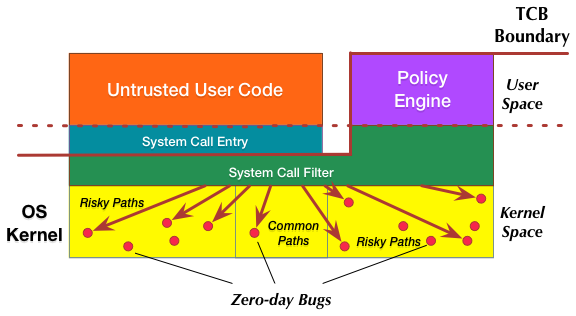
\includegraphics[width=1.0\columnwidth]{diagram/Virtualization_Design_Model_03.png}
\caption{\small Schematic of System Call Interposition.}
\label{fig:design_system_call_interposition}
\end{figure}

SCI was once popular
%approach to the design of secure virtualization systems because
because it gave developers the ability to set and enforce security policies.
%\lois{I think I asked this during the last revision. You say ``was"
%a popular approach. Is it not a popular approach anymore?}
%\yiwen{It is not a popular approach anymore, since no modern design could simply rely on
%this idea to build practical system.}
However, this design is limited by its overly complicated approach to policy
decisions and implementation.
To make a policy decision, the system needs to
obtain and interpret the OS state (e.g., permissions, user groups, register flags)
associated with the programs it is monitoring.
The complexity of OS states makes this process difficult and can lead to
inaccurate policy decisions.
In addition, there are many indirect paths in the kernel that can be accessed.
If security policy makers overlook those paths, it renders the
policy ineffective, as attackers will be able to
bypass the imposed security checks.
Moreover, many side-effects of blocking
certain system calls could affect the function of desired system calls.
It is difficult for developers to fully understand the side-effects of all the
system calls in an interface as complex as the UNIX API.
For example, many applications that rely on \texttt{setuid} fail to check its return value.
If \texttt{setuid} fails, these applications will continue to function in a compromised state,
with incorrect permissions and privileges.
The above limitations make it very challenging to design and build a secure virtualization system using
system call interposition alone.

\subsection{Functionality Re-Creation}
Systems such as  Drawbridge \cite{Drawbridge-11},
 Bascule \cite{Bascule}, and Graphene \cite{Graphene-14} can
provide richer functionality and run more complex programs than most systems built
with SCI because they have their own
interfaces and libraries. Some virtualization
systems, such as OS VM systems VirtualBox, and VMWare Workstation, even have the
full functionalities of an OS re-created in their codebase. We call such a design
``functionality re-creation."

\begin{figure}%[h]
\centering
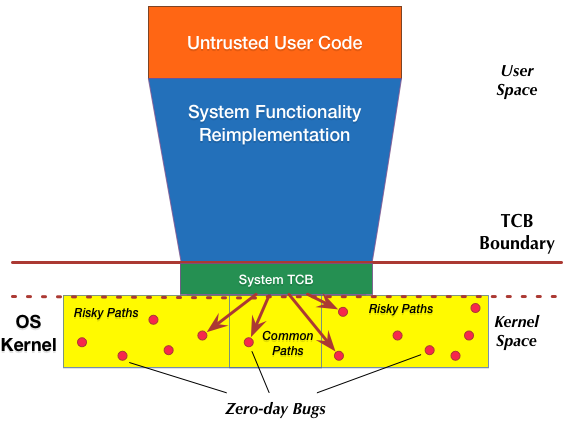
\includegraphics[width=1.0\columnwidth]{diagram/Virtualization_Design_Model_02.png}
\caption{\small Schematic of Functionality Re-creation System.}
\label{fig:design_functionality_reimplementation}
\end{figure}

The key to this design is to not fully rely on the underlying
kernel for system functions. As illustrated in Figure \ref{fig:design_functionality_reimplementation},
this design re-creates its own system functionalities to provide to user code.
When it has to %communicate with the kernel to
access resources like memory, CPU, and disk storage, the system accesses the kernel directly with
its underlying TCB code.
%which can access the kernel directly.
For example, Graphene \cite{Graphene-14} re-creates
its own Linux system calls in
\texttt{libLinux.so}. When it needs to acquire resources from
the kernel, it uses a
Platform Adaptation Layer (PAL)  that has access to the kernel
and provides basic ABI functions to the OS library.

Functionality re-creation provides a more realistic solution to building
virtualization systems than earlier efforts, and offers rich functionality.
However, hundreds of vulnerabilities have been
reported in existing virtualization systems over the past ten years~\cite{NVD}.
One shortcoming of such systems is they often
introduce large codebases and enlarged TCBs. In addition, the
complex semantics of OS functions can easily result in bugs and vulnerabilities
emerging during the re-creation process. Some of these vulnerabilities
can directly cause a privilege escalation, which allows attackers to escape the sandbox
and execute arbitrary code on the host OS.
For example, a vulnerability in VMWare's codebase caused by buffer overflows in the VIX
API allowed local users to escape the guest VM and
gain privilege to execute arbitrary code in the host
OS, even shellcode to access the kernel of the host OS~\cite{CVE-2008-2100}.

Even operations that are considered
legal and harmless in the guest OS may open up risky system call paths in the underlying
host OS and cause a problem.
This type of problem can be fatal,
as it can reach and trigger vulnerabilities in the underlying OS kernel.

\subsection{Lock-in-Pop: Staying on the Beaten Path }
As discussed above, weakness of the previous approaches is the inevitable contact
between the privileged kernel code and the untrusted application.
By leveraging our key observation
that ``popular, frequently-used kernel paths contain fewer bugs," we propose a design
in which all code, including the complex part
of the operating system interface, access only
popular kernel paths through a small TCB. As it ``locks" all functionality
requests into only the ``popular" paths, we dubbed the
design ``Lock-in-Pop."

\begin{figure}%[h]
\centering
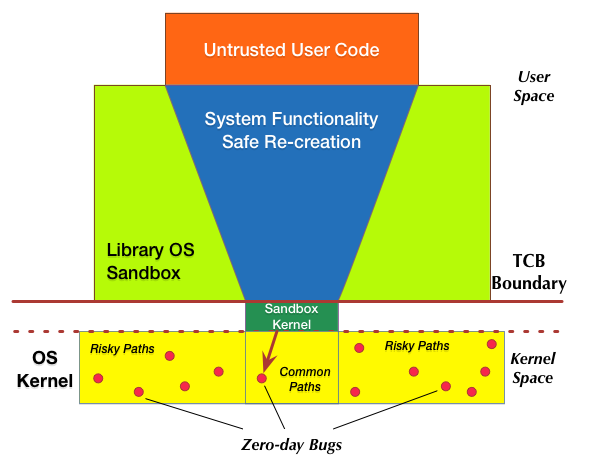
\includegraphics[width=.9\columnwidth]{diagram/Virtualization_Design_Model_01.png}
\caption{\small ``Lock-in-Pop''System ensures safe execution of untrusted user code
despite existing potential zero-day bugs in the OS kernel.}
\label{fig:design_safe_reimplementation}
\end{figure}

In addition, the system is located entirely in the userspace, and both the size of
the sandbox kernel and its access to the OS kernel is restricted
(Figure \ref{fig:design_safe_reimplementation}). Any complex or possibly risky system
functions that require contact with the OS kernel is re-created using
memory-safe code and is contained within a sandbox. This approach has advantages
over others that require modifications to
the OS kernel (Section {\ref{sec.metric}). The isolation provided by placing
``Lock-in-Pop'' in the userspace is also an added protection over the functionality
re-creation modules. Lock-in-Pop does not
expose kernel privileges that could allow attacks
in the underlying system and any applications in the userspace.

As shown in Figure \ref{fig:design_safe_reimplementation}, the key to
``Lock-in-Pop'' is that it constructs a set of safe system functions within
the library OS sandbox.
The sandbox responds to system call requests and
returns results to the user code, if the requests are granted.
It is comprised of two parts: a sandbox kernel that provides access to basic but critical
system calls, and a safely re-created API to implement more
complex calls, such as symbolic link system call.
The sandbox kernel forms the only TCB of our library OS, and is kept
extremely small and simple so that it is easy to verify its security.
The sandbox code provides an API that performs a few critical system calls with
the most basic parameters, such as writing data to the file system
and communicating with the network.
%The kernel utilizes the most simplistic calls
%possible with the most basic arguments.
Complex system functionality is then built on top of the sandbox kernel using our
safer re-creation interface.
The safe re-creation technique of sandbox kernel APIs will then use those basic
resources, such as memory allocations,
network sockets, and file descriptors to construct a more complex virtual system interface, which will be
provided to untrusted user code.

%With the system functionality safe reimplementation, unmodified user code is able to run on top of our designed system.
It is important to note that our design does not rely on any specific technique or tool, and it is possible
to choose from several different techniques that fit specific security requirements.
The following section describes one implementation of our design called Lind.
